\documentclass{article}

\usepackage[margin=1in]{geometry} 
\usepackage{amsmath,amsthm,amssymb,amsfonts, fancyhdr, color, comment, graphicx, environ}
\usepackage{xcolor}
\usepackage{mdframed}
\usepackage[shortlabels]{enumitem}
\usepackage{indentfirst}
\usepackage{hyperref}
\usepackage[spanish]{babel}
\usepackage{pgfplots} % Add this line
\pgfplotsset{compat=1.18}
\usepackage{fancyhdr}
\hypersetup{
    colorlinks=true,
    linkcolor=blue,
    filecolor=magenta,      
    urlcolor=blue,
}
\setlength{\headheight}{1.5cm}
\usepackage{tikz}

\newenvironment{theorem}[2][Teorema]
    { \begin{mdframed}[backgroundcolor=green!20] \textbf{#1 #2} \\}
    {  \end{mdframed}}

\newenvironment{definition}[2][Definición]
    { \begin{mdframed}[backgroundcolor=blue!10] \textbf{#1 #2} \\}
    {  \end{mdframed}}

\newenvironment{lema}[2][Lema]
    { \begin{mdframed}[backgroundcolor=blue!10] \textbf{#1 #2} \\}
    {  \end{mdframed}}

\newenvironment{example}[2][Ejemplo]
    { \begin{mdframed}[backgroundcolor=red!10] \textbf{#1 #2} \\}
    {  \end{mdframed}}

\newenvironment{exercise}[2][Ejercicio]
    { \begin{mdframed}[backgroundcolor=yellow!10] \textbf{#1 #2} \\}
    {  \end{mdframed}}

\newenvironment{remark}[2][Observación]
    { \begin{mdframed}[backgroundcolor=gray!10] \textbf{#1 #2} \\}
    {  \end{mdframed}}

\title{Notas de Clase}
\author{Villar Pedro}
\date{\today}

\pagestyle{fancy}
\fancyhf{}
\rhead{Notas de Clase}
\lhead{\leftmark}
\rfoot{Página \thepage}

\begin{document}
\maketitle
\newpage
\tableofcontents
\newpage
\listoffigures
\newpage
\section[Unidad 4 - Aproximación de Funciones]{Aproximación de funciones}
\subsection[Aproximación con n puntos]{Método de Mínimos Cuadrados}
Supongamos que se tienen $n$ puntos $(x_1, y_1), (x_2, y_2), \dots, (x_n, y_n)$ y se desea encontrar una función $f(x)$ que se ajuste a estos puntos. Se busca una función de la forma $f(x) = a_0 + a_1x + a_2x^2 + \dots + a_mx^m$ tal que la suma de los cuadrados de los errores sea mínima. 
\begin{figure}[h]
    \centering
    \begin{tikzpicture}
        \begin{axis}[
            xlabel={$x$},
            ylabel={$y$},
            xmin=-5, xmax=5,
            ymin=-5, ymax=5,
            axis lines=center,
            axis on top=true,
            domain=-5:5,
            ]
            \addplot [mark=none,draw=blue] {x};
            \addplot [only marks, mark=*, draw=green] coordinates {(1,1.1) (2,2.14) (3,2.9) (1.5, 1.6) (0.5, 0.47) (2.5, 2.38)};
        \end{axis}
    \end{tikzpicture}
    \caption{Ejemplo de Aproximación}
    \label{fig:myplot}
\end{figure}
Suponiendo que la función $f(x)$ es de la forma $ax+b$, se tiene que la suma de los cuadrados de los errores es
\begin{equation}
    E(a,b) = \sum_{i=1}^{n} (y_i - (ax_i + b))^2
\end{equation}
luego, derivando con respecto a $a$ y $b$ e igualando a cero se obtiene el sistema de ecuaciones
\begin{align}
    \frac{\partial E}{\partial a} &= -2\sum_{i=1}^{n} x_i(y_i - (ax_i + b)) = 0 \\
    \frac{\partial E}{\partial b} &= -2\sum_{i=1}^{n} (y_i - (ax_i + b)) = 0
\end{align}
reordenando estas ecuaciones se pueden obtener las \textbf{ecuaciones normales}:
\begin{align}
    a &= \frac{n\sum_{i=1}^{n} x_iy_i - \sum_{i=1}^{n} x_i \sum_{i=1}^{n} y_i}{n\sum_{i=1}^{n} x_i^2 - (\sum_{i=1}^{n} x_i)^2} \\
    b &= \frac{(\sum_{i=1}^{n} y_i)\sum_{i=1}^{n} x_i^2 - (\sum_{i=1}^{n} x_i)(\sum_{i=1}^{n} x_iy_i)}{n\sum_{i=1}^{n} x_i^2 - (\sum_{i=1}^{n} x_i)^2}
\end{align}
\newpage
\subsubsection{Método de Solución del sistema}
\begin{theorem}{Teorema de la Transpuesta}
    Dado un sistema de ecuaciones lineales $Ax = b$, se puede resolver el sistema de ecuaciones utilizando la matriz transpuesta de $A$ de la siguiente forma:
    \begin{equation}
        A^TAx = A^Tb
    \end{equation}
\end{theorem}
Basándonos en el teorema anterior, se puede resolver el sistema de ecuaciones de la siguiente forma, tomando una base de funciones de grado 1: $\mathcal{B} = \{1, x\}$, podemos plantear las siguientes matrices $A$, $x$ y $b$:
\begin{equation}
    A = \begin{bmatrix}
        x_1 & 1 \\
        x_2 & 1 \\
        \vdots & \vdots \\
        x_n & 1
    \end{bmatrix}, \quad x = \begin{bmatrix}
        a \\
        b
    \end{bmatrix}, \quad b = \begin{bmatrix}
        y_1 \\
        y_2 \\
        \vdots \\
        y_n
    \end{bmatrix}
\end{equation}
luego, se puede resolver el sistema de ecuaciones $Ax = b$ de la siguiente forma:
\begin{equation}
    A^TAx = A^Tb
\end{equation}
\begin{equation}
    \begin{bmatrix}
        \sum_{i=1}^{n} x_i^2 & \sum_{i=1}^{n} x_i \\
        \sum_{i=1}^{n} x_i & n
    \end{bmatrix} \begin{bmatrix}
        a \\
        b
    \end{bmatrix} = \begin{bmatrix}
        \sum_{i=1}^{n} x_iy_i \\
        \sum_{i=1}^{n} y_i
    \end{bmatrix}
\end{equation}
La solución de este sistema de ecuaciones, nos da la forma de armar la función $f(x) = ax + b$ que mejor se ajusta a los puntos dados.
De forma análoga, si se busca una función de grado 2, se puede plantear el sistema de ecuaciones de la siguiente forma:
\begin{equation}
    A = \begin{bmatrix}
        x_1^2 & x_1 & 1 \\
        x_2^2 & x_2 & 1 \\
        \vdots & \vdots & \vdots \\
        x_n^2 & x_n & 1
    \end{bmatrix}, \quad x = \begin{bmatrix}
        a \\
        b \\
        c
    \end{bmatrix}, \quad b = \begin{bmatrix}
        y_1 \\
        y_2 \\
        \vdots \\
        y_n
    \end{bmatrix}
\end{equation}
luego, se puede resolver el sistema de ecuaciones $Ax = b$ de la siguiente forma:
\begin{equation}
    A^TAx = A^Tb
\end{equation}
\begin{equation}
    \begin{bmatrix}
        \sum_{i=1}^{n} x_i^4 & \sum_{i=1}^{n} x_i^3 & \sum_{i=1}^{n} x_i^2 \\
        \sum_{i=1}^{n} x_i^3 & \sum_{i=1}^{n} x_i^2 & \sum_{i=1}^{n} x_i \\
        \sum_{i=1}^{n} x_i^2 & \sum_{i=1}^{n} x_i & n
    \end{bmatrix} \begin{bmatrix}
        a \\
        b \\
        c
    \end{bmatrix} = \begin{bmatrix}
        \sum_{i=1}^{n} x_i^2y_i \\
        \sum_{i=1}^{n} x_iy_i \\
        \sum_{i=1}^{n} y_i
    \end{bmatrix}
\end{equation}
La solución de este sistema de ecuaciones, nos da la forma de armar la función $f(x) = ax^2 + bx + c$ que mejor se ajusta a los puntos dados.

Principalmente este sistema se basa en expresar como un polinomio, el tipo de función que se quiera usar de aproximación principalmente aplicando logaritmo natural de ambos lados, por ejemplo:
\begin{equation}
    f(x) = ae^{bx} \Rightarrow \ln(f(x)) = \ln(a) + bx
\end{equation}
\subsection{Ejercicios Guía 4}
\subsubsection{Ejercicio 1}
\noindent \textbf{a)} Encuentre el polinomio de grado $1$ que aproxima en el sentido de cuadrados m\'inimos la siguiente tabla de datos:
\begin{center}
\begin{tabular}{||r||r|r|r|r|r|r|r|r|r|r||}
\hline
x & 0 & 1 & 2 & 3 & 4 & 5 & 6 & 7 & 8 & 9 \\
y & -0.1 & 1.1 & 1.9 & 3.2 & 3.8 & 5.0 & 6.0 & 7.3 & 8.1 & 8.9 \\
\hline
\end{tabular}
\end{center}
\textbf{b)} y el polinomio de grado $2$ que aproxima en el mismo sentido la siguiente tabla de datos:
\begin{center}
\begin{tabular}{||r||r|r|r|r|r||}
\hline
x & -1 & 0 & 1 & 3 & 6 \\
y & 6.1 & 2.8 & 2.2 & 6 & 26.9 \\
\hline
\end{tabular}
\end{center}
Para resolver este ejercicio, se puede plantear el sistema de ecuaciones $Ax = b$ y resolverlo utilizando el teorema de la transpuesta.
\begin{center}
    Punto a) $f(x) = ax + b$ \\
\end{center}
\begin{equation}
    A = \begin{bmatrix}
        0 & 1 \\
        1 & 1 \\
        2 & 1 \\
        3 & 1 \\
        4 & 1 \\
        5 & 1 \\
        6 & 1 \\
        7 & 1 \\
        8 & 1 \\
        9 & 1
    \end{bmatrix}, \quad x = \begin{bmatrix}
        a \\
        b
    \end{bmatrix}, \quad b = \begin{bmatrix}
        -0.1 \\
        1.1 \\
        1.9 \\
        3.2 \\
        3.8 \\
        5.0 \\
        6.0 \\
        7.3 \\
        8.1 \\
        8.9
    \end{bmatrix}
\end{equation}
El resultado de resolver el sistema aplicando el teorema es:
\begin{equation}
    A^TA = \begin{bmatrix}
        285 & 45 \\
        45 & 10
    \end{bmatrix}, \quad A^Tb = \begin{bmatrix}
        \frac{2867}{10} \\
        \frac{226}{5}
    \end{bmatrix}
\end{equation}
El resultado de resolver el sistema de ecuaciones es:
\begin{equation}
    a = \frac{833}{825}, \quad b = -\frac{13}{550}
\end{equation}
Y por lo tanto, la función que mejor se ajusta a los puntos dados es:
\begin{equation}
    f(x) = \frac{833}{825}x - \frac{13}{550}
\end{equation}
\begin{figure}[h]
    \centering
    \begin{tikzpicture}
        \begin{axis}[
            xlabel={$x$},
            ylabel={$y$},
            xmin=-1, xmax=10,
            ymin=-1, ymax=10,
            axis lines=center,
            axis on top=true,
            domain=-1:10,
            ]
            \addplot [mark=none,draw=blue] {(833/825)*x - (13/550)};
            \addplot [only marks, mark=*, draw=green] coordinates {(0,-0.1) (1,1.1) (2,1.9) (3,3.2) (4,3.8) (5,5.0) (6,6.0) (7,7.3) (8,8.1) (9,8.9)};
        \end{axis}
    \end{tikzpicture}
    \caption{Aproximación de la función $f(x) = \frac{833}{825}x - \frac{13}{550}$}
    \label{fig:myplot2}
\end{figure}
\begin{center}
    Punto b) $f(x) = ax^2 + bx + c$ \\
\end{center}
\begin{equation}
    A = \begin{bmatrix}
        1 & -1 & 1 \\
        0 & 0 & 1 \\
        1 & 1 & 1 \\
        9 & 3 & 1 \\
        36 & 6 & 1
    \end{bmatrix}, \quad x = \begin{bmatrix}
        a \\
        b \\
        c
    \end{bmatrix}, \quad b = \begin{bmatrix}
        6.1 \\
        2.8 \\
        2.2 \\
        6 \\
        26.9
    \end{bmatrix}
\end{equation}
El resultado de resolver el sistema aplicando el teorema es:
\begin{equation}
    A^TA = \begin{bmatrix}
        1379 & 243 & 47 \\
        243 & 47 & 5 \\
        47 & 9 & 5
    \end{bmatrix}, \quad A^Tb = \begin{bmatrix}
        \frac{10307}{10} \\
        \frac{351}{2} \\
        44
    \end{bmatrix}
\end{equation}
El resultado de resolver el sistema de ecuaciones es:
\begin{equation}
    a = \frac{2843}{2860}, \quad b = -\frac{5679}{2860}, \quad c = \frac{4333}{1430}
\end{equation}
Y por lo tanto, la función que mejor se ajusta a los puntos dados es:
\begin{equation}
    f(x) = \frac{2843}{2860}x^2 - \frac{5679}{2860}x + \frac{4333}{1430}
\end{equation}
\begin{figure}[h]
    \centering
    \begin{tikzpicture}
        \begin{axis}[
            xlabel={$x$},
            ylabel={$y$},
            xmin=-1, xmax=10,
            ymin=-1, ymax=30,
            axis lines=center,
            axis on top=true,
            domain=-1:10,
            ]
            \addplot [mark=none,draw=blue] {(2843/2860)*x^2 - (5679/2860)*x + (4333/1430)};
            \addplot [only marks, mark=*, draw=green] coordinates {(-1,6.1) (0,2.8) (1,2.2) (3,6) (6,26.9)};
        \end{axis}
    \end{tikzpicture}
    \caption{Aproximación de la función $f(x) = \frac{2843}{2860}x^2 - \frac{5679}{2860}x + \frac{4333}{1430}$}
    \label{fig:myplot3}
\end{figure}
\subsubsection{Ejercicio 2}
Pruebe que si se tienen $n+1$ puntos distintos, la aproximación polinomial de grado $n$ (en el sentido de cuadrados mínimos)  coincide con el polinomio interpolatorio. Observe que esto implicaría que la aproximación polinomial en el sentido de cuadrados mínimos tendría grado alto (en caso que $n$ sea grande) y esto no es aconsejable.

Para demostrar que la aproximación polinomial de grado \( n \) en el sentido de cuadrados mínimos coincide con el polinomio interpolatorio cuando se tienen \( n+1 \) puntos distintos, consideremos los siguientes pasos:
\begin{center}
    \textbf{1. Polinomio Interpolatorio de Lagrange}
\end{center}

Dado un conjunto de \( n+1 \) puntos distintos \((x_i, y_i)\) para \( i = 0, 1, \ldots, n \), el polinomio interpolatorio \( P(x) \) de grado \( n \) que pasa exactamente por estos puntos se puede expresar como:
\[
P(x) = \sum_{i=0}^{n} y_i \ell_i(x),
\]
donde los polinomios base de Lagrange \( \ell_i(x) \) están definidos por:
\[
\ell_i(x) = \prod_{\substack{j=0 \\ j \neq i}}^{n} \frac{x - x_j}{x_i - x_j}.
\]
\newpage
\begin{center}
    \textbf{2. Aproximación Polinomial en el Sentido de Cuadrados Mínimos}
\end{center}

El objetivo de la aproximación polinomial en el sentido de cuadrados mínimos es encontrar un polinomio \( Q(x) \) de grado \( n \) que minimice la suma de los cuadrados de las diferencias entre los valores observados \( y_i \) y los valores predichos \( Q(x_i) \):
\[
\sum_{i=0}^{n} \left( y_i - Q(x_i) \right)^2.
\]

Para encontrar este polinomio \( Q(x) \), se deben resolver las siguientes ecuaciones normales:
\[
\sum_{i=0}^{n} Q(x_i) \ell_j(x_i) = \sum_{i=0}^{n} y_i \ell_j(x_i) \quad \text{para } j = 0, 1, \ldots, n,
\]
donde \( \ell_j(x) \) son los mismos polinomios base que en la interpolación de Lagrange.

\begin{center}
    \textbf{3. Coincidencia de los Polinomios}
\end{center}

Para probar que el polinomio interpolatorio y el polinomio de cuadrados mínimos coinciden, notamos lo siguiente:
\begin{itemize}
    \item 1. \textbf{Existencia y Unicidad}: Ambos polinomios, \( P(x) \) y \( Q(x) \), son únicos para un conjunto dado de \( n+1 \) puntos distintos.
    \item 2. \textbf{Grado del Polinomio}: Ambos polinomios son de grado \( n \).
    \item 3. \textbf{Condiciones de Interpolación}: El polinomio interpolatorio \( P(x) \) pasa exactamente por todos los puntos \((x_i, y_i)\), y debido a que tiene grado \( n \), esto significa que satisface las \( n+1 \) condiciones de interpolación \( P(x_i) = y_i \).
\end{itemize}


Dado que \( P(x) \) ya satisface estas condiciones de minimización exacta (es decir, pasa exactamente por cada punto \( (x_i, y_i) \)), se puede concluir que el polinomio \( P(x) \) es también la solución al problema de mínimos cuadrados. Así, el polinomio de cuadrados mínimos \( Q(x) \) debe coincidir con el polinomio interpolatorio \( P(x) \).

Por lo tanto, \( P(x) = Q(x) \), demostrando que la aproximación polinomial de grado \( n \) en el sentido de cuadrados mínimos coincide con el polinomio interpolatorio cuando se tienen \( n+1 \) puntos distintos.

\subsubsection{Ejercicio 3}
Halle el polinomio de grado cero que mejor aproxime en el sentido de cuadrados m\'inimos a una funci\'on $f:[a,b]\rightarrow\mathbb{R}$ en $n$ puntos $x_1,\ldots, x_n$ del intervalo $[a,b]$.
Para hallar el polinomio de grado cero que mejor aproxime en el sentido de cuadrados mínimos a una función \( f:[a,b] \rightarrow \mathbb{R} \) en \( n \) puntos \( x_1, \ldots, x_n \) del intervalo \([a,b]\), consideremos el siguiente procedimiento:
\begin{center}
    \textbf{1. Definición del Problema}
\end{center}

Queremos encontrar un polinomio de grado cero \( p(x) = c \) que minimice la suma de los cuadrados de las diferencias entre los valores de \( f \) en los puntos \( x_i \) y \( c \). Es decir, queremos minimizar la siguiente función de error:
\[
E(c) = \sum_{i=1}^n (f(x_i) - c)^2.
\]
\begin{center}
    \textbf{2. Minimización del Error}    
\end{center}


Para encontrar el valor de \( c \) que minimiza \( E(c) \), derivamos \( E(c) \) con respecto a \( c \) y establecemos la derivada igual a cero:
\[
\frac{dE(c)}{dc} = \frac{d}{dc} \left( \sum_{i=1}^n (f(x_i) - c)^2 \right) = \sum_{i=1}^n \frac{d}{dc} (f(x_i) - c)^2.
\]

Usando la regla de la cadena, obtenemos:
\[
\frac{d}{dc} (f(x_i) - c)^2 = 2 (f(x_i) - c)(-1) = -2 (f(x_i) - c).
\]

Por lo tanto, la derivada de \( E(c) \) es:
\[
\frac{dE(c)}{dc} = -2 \sum_{i=1}^n (f(x_i) - c).
\]

Para encontrar el mínimo, establecemos la derivada igual a cero:
\[
-2 \sum_{i=1}^n (f(x_i) - c) = 0.
\]

Esto se simplifica a:
\[
\sum_{i=1}^n (f(x_i) - c) = 0,
\]
\[
\sum_{i=1}^n f(x_i) - n c = 0,
\]
\[
n c = \sum_{i=1}^n f(x_i),
\]
\[
c = \frac{1}{n} \sum_{i=1}^n f(x_i).
\]

El polinomio de grado cero que mejor aproxima en el sentido de cuadrados mínimos a la función \( f \) en los puntos \( x_1, \ldots, x_n \) es:
\[
p(x) = \frac{1}{n} \sum_{i=1}^n f(x_i).
\]

\subsubsection{Ejercicio 4}
Aproximar los datos de la siguiente tabla con un modelo de la forma $f(x) \sim ae^{bx}$ en el sentido de cuadrados mínimos.
\begin{center}
\begin{tabular}{||r||r|r|r|r||}
\hline
x & -1 & 0 & 1 & 2\\
y & 8.1 & 3 & 1.1 & 0.5\\
\hline
\end{tabular}
\end{center}
Para aproximar los datos de la tabla con un modelo de la forma \( f(x) \sim ae^{bx} \) en el sentido de cuadrados mínimos, considero convertir la función a un polinomio, aplicando logaritmo natural a ambos lados:
\[
f(x) = ae^{bx} \Rightarrow \ln(f(x)) = \ln(a) + bx.
\]
Entonces hay que aplicar dicha transformación y en vez de tener $y$ en la tabla, se tiene $\overline{y} = \ln(y)$, por lo que la tabla se convierte en:
\begin{center}
\begin{tabular}{||r||r|r|r|r||}
\hline
x & -1 & 0 & 1 & 2\\
$\overline{y}$ & 2.091864 & 1.098612 & 0.095310 & -0.693147\\
\hline
\end{tabular}
\end{center}
Luego, se puede plantear el sistema de ecuaciones $Ax = b$ y resolverlo utilizando el teorema de la transpuesta.
\begin{equation}
    A = \begin{bmatrix}
        -1 & 1 \\
        0 & 1 \\
        1 & 1 \\
        2 & 1
    \end{bmatrix}, \quad x = \begin{bmatrix}
        b \\
        \ln(a)
    \end{bmatrix}, \quad b = \begin{bmatrix}
        2.091864 \\
        1.098612 \\
        0.095310 \\
        -0.693147
    \end{bmatrix}
\end{equation}
El resultado de resolver los productos es:
\begin{equation}
    A^TA = \begin{bmatrix}
        6 & 2 \\
        2 & 4
    \end{bmatrix}, \quad A^Tb = \begin{bmatrix}
        -3.4 \\
        2.58
    \end{bmatrix}
\end{equation}
El resultado de resolver el sistema de ecuaciones es:
\begin{equation}
    b = -0.938, \quad \ln(a) = 1.114 \Rightarrow a = 3.046
\end{equation}
Y por lo tanto, la función que mejor se ajusta a los puntos dados es:
\begin{equation}
    f(x) = 3.046e^{-0.938x}
\end{equation}
\begin{figure}[h]
    \centering
    \begin{tikzpicture}
        \begin{axis}[
            xlabel={$x$},
            ylabel={$y$},
            xmin=-1, xmax=2,
            ymin=0, ymax=10,
            axis lines=center,
            axis on top=true,
            domain=-1:2,
            ]
            \addplot [mark=none,draw=blue] {3.046*exp(-0.938*x)};
            \addplot [only marks, mark=*, draw=green] coordinates {(-1,8.1) (0,3) (1,1.1) (2,0.5)};
        \end{axis}
    \end{tikzpicture}
    \caption{Aproximación de la función $f(x) = 3.046e^{-0.938x}$}
    \label{fig:myplot4}
\end{figure}

\subsubsection{Ejercicio 5}
Aproximar los datos de la siguiente tabla con un modelo de la forma $f(x) \sim -e^{ax^2+bx+c}$ en el sentido de cuadrados mínimos.
\begin{center}
\begin{tabular}{||r||r|r|r|r||}
\hline
x & -1 & 0 & 1 & 2\\
y & -1.1 & -0.4 & -0.9 & -0.5\\
\hline
\end{tabular}
\end{center}
Para aproximar los datos de la tabla con un modelo de la forma \( f(x) \sim -e^{ax^2+bx+c} \) en el sentido de cuadrados mínimos, considero convertir la función a un polinomio, aplicando logaritmo natural a ambos lados:
\[
f(x) = -e^{ax^2+bx+c} \Rightarrow \ln(-f(x)) = ax^2 + bx + c.
\]
Entonces hay que aplicar dicha transformación y en vez de tener \( y \) en la tabla, se tiene \( \overline{y} = \ln(-y) \), por lo que la tabla se convierte en:
\begin{center}
\begin{tabular}{||r||r|r|r|r||}
\hline
x & -1 & 0 & 1 & 2\\
$\overline{y}$ & 0.09 & -0.91 & -0.10 & -0.69\\
\hline
\end{tabular}
\end{center}
Luego, se puede plantear el sistema de ecuaciones \( Ax = b \) y resolverlo utilizando el teorema de la transpuesta.
\begin{equation}
    A = \begin{bmatrix}
        1 & -1 & 1 \\
        0 & 0 & 1 \\
        1 & 1 & 1 \\
        4 & 2 & 1
    \end{bmatrix}, \quad x = \begin{bmatrix}
        a \\
        b \\
        c
    \end{bmatrix}, \quad b = \begin{bmatrix}
        0.09 \\
        -0.91 \\
        -0.10 \\
        -0.69
    \end{bmatrix}
\end{equation}
El resultado de resolver los productos es:
\begin{equation}
    A^TA = \begin{bmatrix}
        18 & 8 & 6 \\
        8 & 6 & 2 \\
        6 & 2 & 4
    \end{bmatrix}, \quad A^Tb = \begin{bmatrix}
        -2.77 \\
        -1.57 \\
        -1.61
    \end{bmatrix}
\end{equation}
El resultado de resolver el sistema de ecuaciones es:
\begin{equation}
    a = 0.41, \quad b = -0.25, \quad c = -0.85
\end{equation}
Y por lo tanto, la función que mejor se ajusta a los puntos dados es:
\begin{equation}
    f(x) = -e^{0.41x^2 - 0.25x - 0.85}
\end{equation}
\begin{figure}[h]
    \centering
    \begin{tikzpicture}
        \begin{axis}[
            xlabel={$x$},
            ylabel={$y$},
            xmin=-1, xmax=2,
            ymin=-2, ymax=2,
            axis lines=center,
            axis on top=true,
            domain=-1:2,
            ]
            \addplot [mark=none,draw=blue] {-exp(0.41*x^2 - 0.25*x - 0.85)};
            \addplot [only marks, mark=*, draw=green] coordinates {(-1,-1.1) (0,-0.4) (1,-0.9) (2,-0.5)};
        \end{axis}
    \end{tikzpicture}
    \caption{Aproximación de la función \( f(x) = -e^{0.41x^2 - 0.25x - 0.85} \)}
    \label{fig:myplot5}
\end{figure}
\begin{remark}
    La aproximación no es la mejor, una mejor manera de aproximar seria usando el modelo de $f(x) \sim -e^{ax^3+bx^2+cx+d}$, ya que el modelo de $f(x) \sim -e^{ax^2+bx+c}$ no se ajusta de la mejor manera a los datos.    
\end{remark}

\subsubsection{Ejercicio 6}
Suponer que se realizó un experimento para encontrar la constante de elasticidad $k$ de la Ley de Hooke: $F= k(l-5.3)$. La función $F$ es la fuerza requerida para estirar el resorte $l$ unidades.
\begin{itemize}
    \item[a) ] Se midieron las fuerzas $F(l)$ para distintas longitudes $l$ y se obtuvo la siguiente tabla:
    \begin{center}
        \begin{tabular}{||r||r|r|r||}
        \hline
        l & 7 & 9.4 & 12.3 \\
        F & 2 & 4 & 5 \\
        \hline
        \end{tabular}
    \end{center}
    Encontrar la mejor aproximación en el sentido de cuadrados mínimos para la constante de elasticidad $k$.
    \item[b) ] Realizando más mediciones se obtuvieron nuevos datos
    \begin{center}
        \begin{tabular}{||r||r|r|r|r||}
        \hline
        l & 8.3 & 11.3 & 14.4 & 15.9 \\
        F & 3 & 5 & 8 & 10 \\
        \hline
        \end{tabular}  
    \end{center}
    Calcular la nueva aproximación para $k$ sólo con el segundo grupo de valores.
    \item[c) ] ¿Cuál valor de $k$ aproxima mejor utilizando los datos de todas las mediciones?
\end{itemize}

\begin{center}
    Punto a) \\
\end{center}

Para encontrar la mejor aproximación en el sentido de cuadrados mínimos para la constante de elasticidad \( k \) con los datos dados, primero convertimos la ecuación de la Ley de Hooke a una forma lineal, tomando como $x$ a $l-5.3$, se forma la tabla:
\begin{center}
    \begin{tabular}{||r||r|r|r||}
    \hline
    x & 1.7 & 4.1 & 7 \\
    F & 2 & 4 & 5 \\
    \hline
    \end{tabular}
\end{center}
Luego, se puede plantear el sistema de ecuaciones \( Ax = b \) y resolverlo utilizando el teorema de la transpuesta.
\begin{equation}
    A = \begin{bmatrix}
        1.7 & 1 \\
        4.1 & 1 \\
        7 & 1
    \end{bmatrix}, \quad x = \begin{bmatrix}
        k \\
        -5.3k
    \end{bmatrix}, \quad b = \begin{bmatrix}
        2 \\
        4 \\
        5
    \end{bmatrix}
\end{equation}
El resultado de resolver los productos es:
\begin{equation}
    A^TA = \begin{bmatrix}
        68.7 & 12.8 \\
        12.8 & 3
    \end{bmatrix}, \quad A^Tb = \begin{bmatrix}
        54.8 \\
        11
    \end{bmatrix}
\end{equation}
El resultado de resolver el sistema de ecuaciones es:
\begin{equation}
    k = 0.80
\end{equation}
Y por lo tanto, la constante de elasticidad \( k \) que mejor se ajusta a los puntos dados es:
\begin{equation}
    k = 0.80
\end{equation}
Visualizando la aproximación:
\begin{figure}[h]
    \centering
    \begin{tikzpicture}
        \begin{axis}[
            xlabel={$l$},
            ylabel={$F$},
            xmin=7, xmax=13,
            ymin=0, ymax=6,
            axis lines=center,
            axis on top=true,
            domain=7:13,
            ]
            \addplot [mark=none,draw=blue] {0.80*(x-5.3)};
            \addplot [only marks, mark=*, draw=green] coordinates {(7,2) (9.4,4) (12.3,5)};
        \end{axis}
    \end{tikzpicture}
    \caption{Aproximación de la constante de elasticidad \( k = 0.80 \)}
    \label{fig:myplot6}
\end{figure}

\begin{center}
    Punto b) \\
\end{center}

Para calcular la nueva aproximación para \( k \) sólo con el segundo grupo de valores, primero convertimos la ecuación de la Ley de Hooke a una forma lineal, tomando como \( x \) a \( l-5.3 \), se forma la tabla:
\begin{center}
    \begin{tabular}{||r||r|r|r|r||}
    \hline
    x & 2.9 & 6 & 9.1 & 10.6 \\
    F & 3 & 5 & 8 & 10 \\
    \hline
    \end{tabular}
\end{center}

Luego, se puede plantear el sistema de ecuaciones \( Ax = b \) y resolverlo utilizando el teorema de la transpuesta.
\begin{equation}
    A = \begin{bmatrix}
        2.9 & 1 \\
        6 & 1 \\
        9.1 & 1 \\
        10.6 & 1
    \end{bmatrix}, \quad x = \begin{bmatrix}
        k \\
        -5.3k
    \end{bmatrix}, \quad b = \begin{bmatrix}
        3 \\
        5 \\
        8 \\
        10
    \end{bmatrix}
\end{equation}
El resultado de resolver los productos es:
\begin{equation}
    A^TA = \begin{bmatrix}
        239.58 & 28.6 \\
        28.6 & 4
    \end{bmatrix}, \quad A^Tb = \begin{bmatrix}
        217.5 \\
        26
    \end{bmatrix}
\end{equation}
El resultado de resolver el sistema de ecuaciones es:
\begin{equation}
    k = 0.90
\end{equation}
Y por lo tanto, la constante de elasticidad \( k \) que mejor se ajusta a los puntos dados es:
\begin{equation}
    k = 0.90
\end{equation}
Visualizando la aproximación:
\begin{figure}[h]
    \centering
    \begin{tikzpicture}
        \begin{axis}[
            xlabel={$l$},
            ylabel={$F$},
            xmin=8, xmax=16,
            ymin=0, ymax=12,
            axis lines=center,
            axis on top=true,
            domain=8:16,
            ]
            \addplot [mark=none,draw=blue] {0.90*(x-5.3)};
            \addplot [only marks, mark=*, draw=green] coordinates {(8.3,3) (11.3,5) (14.4,8) (15.9,10)};
        \end{axis}
    \end{tikzpicture}
    \caption{Aproximación de la constante de elasticidad \( k = 0.90 \)}
    \label{fig:myplot7}
\end{figure}

\begin{center}
    Punto c) \\
\end{center}

Para encontrar el valor de \( k \) que aproxima mejor utilizando los datos de todas las mediciones, primero convertimos la ecuación de la Ley de Hooke a una forma lineal, tomando como \( x \) a \( l-5.3 \), se forma la tabla:
\begin{center}
    \begin{tabular}{||r||r|r|r|r|r|r|r|r||}
    \hline
    x & 1.7 & 4.1 & 7 & 2.9 & 6 & 9.1 & 10.6 \\
    F & 2 & 4 & 5 & 3 & 5 & 8 & 10 \\
    \hline
    \end{tabular}
\end{center}
Luego, se puede plantear el sistema de ecuaciones \( Ax = b \) y resolverlo utilizando el teorema de la transpuesta.
\begin{equation}
    A = \begin{bmatrix}
        1.7 & 1 \\
        4.1 & 1 \\
        7 & 1 \\
        2.9 & 1 \\
        6 & 1 \\
        9.1 & 1 \\
        10.6 & 1
    \end{bmatrix}, \quad x = \begin{bmatrix}
        k \\
        -5.3k
    \end{bmatrix}, \quad b = \begin{bmatrix}
        2 \\
        4 \\
        5 \\
        3 \\
        5 \\
        8 \\
        10
    \end{bmatrix}
\end{equation}
El resultado de resolver los productos es:
\begin{equation}
    A^TA = \begin{bmatrix}
        308.28 & 41.4 \\
        41.4 & 7
    \end{bmatrix}, \quad A^Tb = \begin{bmatrix}
        272.3 \\
        37
    \end{bmatrix}
\end{equation}
El resultado de resolver el sistema de ecuaciones es:
\begin{equation}
    k = 0.84
\end{equation}
Y por lo tanto, la constante de elasticidad \( k \) que mejor se ajusta a todos los puntos dados es:
\begin{equation}
    k = 0.84
\end{equation}
Visualizando la aproximación:
\begin{figure}[h]
    \centering
    \begin{tikzpicture}
        \begin{axis}[
            xlabel={$l$},
            ylabel={$F$},
            xmin=7, xmax=16,
            ymin=0, ymax=12,
            axis lines=center,
            axis on top=true,
            domain=7:16,
            ]
            \addplot [mark=none,draw=blue] {0.84*(x-5.3)};
            \addplot [only marks, mark=*, draw=green] coordinates {(7,2) (9.4,4) (12.3,5) (8.3,3) (11.3,5) (14.4,8) (15.9,10)};
        \end{axis}
    \end{tikzpicture}
    \caption{Aproximación de la constante de elasticidad \( k = 0.84 \)}
    \label{fig:myplot8}
\end{figure}

\subsection[Aproximación con infinitos puntos]{Método de aproximación con infinitos puntos}
Ahora el problema pasa a ser, encontrar el mejor polinomio de grado $n$ que mejor aproxima a una función $f(x)$ en un intervalo $[a,b]$. Para ello, se puede plantear el problema de minimización de la siguiente manera:
\begin{equation}
    E_2(a_0,a_1,\dots,a_n) = \int_{a}^{b} (f(x) - p(x))^2 dx
\end{equation}
En este caso, las ecuaciones normales son:
\begin{equation}
    \sum_{k=0}^{n} a_k \int_{a}^{b} x^{k+j} dx = \int_{a}^{b} f(x)x^j dx
\end{equation}
para $j=0,1,\dots,n$. Luego, se puede resolver el sistema de ecuaciones para encontrar los coeficientes $a_0,a_1,\dots,a_n$.

Al plantear este sistema, se forma una matriz de \textbf{Hilbert} de tamaño $n+1$:
\begin{equation}
    H_{ij} = \int_{a}^{b} x^{i+j} dx = \frac{b^{i+j+1} - a^{i+j+1}}{i+j+1}
\end{equation}
La matriz de \textbf{Hilbert} tiene el problema de que es mala, entonces si se quiere encontrar las soluciones de el sistema de ecucaciones $Hx=b$ una buena opción es llegar de alguna forma a que la matriz sea la identidad.
\begin{definition}{Función peso}
    Una función integrable $\omega(x)$ se llama \textbf{función de peso} en el intervalo $I$ si $\omega(x) > 0$ para todo $x \in I$, pero $\omega \neq 0$ para todo $x$ en cualquier subintervalo de $I$, es decir $\omega(x)$ no puede ser constantemente $0$ en un intervalo.
\end{definition}

\begin{definition}{Polinomios ortogonales con peso}
    Un conjunto $\{ \phi_0, \phi_1, \dots, \phi_n \}$ de polinomios que:
    \begin{equation}
        gr(\phi_k) = k
        \label{eq:ecuacion45}
    \end{equation}
    \begin{equation}
        \int_{a}^{b} \omega(x) \phi_k(x) \phi_j(x) dx = 
        \begin{cases}
            0 & \text{si } k \neq j \\
            \alpha_j & \text{si } k = j
        \end{cases}
        \label{eq:ecuacion46}
    \end{equation}
    se llaman \textbf{polinomios ortogonales con peso} $\omega(x)$ en el intervalo $[a,b]$.
\end{definition}

\begin{lema}{Linealidad de los polinomios ortogonales con peso}
    Si $\{ \phi_0, \phi_1, \dots, \phi_n \}$ son polinomios ortogonales con peso $\omega(x)$ en el intervalo $[a,b]$, entonces son linealmente independientes.
\end{lema}

\begin{definition}{Familia de polinomios ortogonales con peso}
    Una familia de polinomios ortogonales con peso $\omega(x)$ en el intervalo $[a,b]$ es un conjunto de polinomios $\{ \phi_0, \phi_1, \dots, \phi_n \}$ que satisface la condición de ortogonalidad. (ver: \ref{eq:ecuacion45} y \ref{eq:ecuacion46})
\end{definition}

\begin{lema}{Ortogonalidad}
    Si $Q_k(x)$ es un polinomio de grado $k<n$ y $\{ \phi_0, \phi_1, \dots, \phi_n \}$ es una familia de polinomios ortogonales con peso $\omega(x)$ en el intervalo $[a,b]$, entonces:
    \begin{equation}
        \langle Q_k, \phi_j \rangle = 0
    \end{equation}
    para $k\neq j$.
\end{lema}

\begin{theorem}
    El conjunto de polinomios $\{ \phi_0, \phi_1, \dots, \phi_n \}$ definido como:
    \begin{align}
        \phi_0(x) &= 1 \\
        \phi_1(x) &= x - B_1 \\
    \end{align}
    donde 
    \begin{equation}
        B_1 = \frac{\int_{a}^{b} x \omega(x) \phi_0^2(x) dx}{\int_{a}^{b} w(x)\phi_0^2(x) dx} \quad \text{ y } \quad \phi_k(x) = (x - B_k) \phi_{k-1}(x) - C_k \phi_{k-2}(x)
    \end{equation}
    donde
    \begin{equation}
        B_k = \frac{\int_{a}^{b} x \omega(x) \phi_{k-1}^2(x) dx}{\int_{a}^{b} w(x)\phi_{k-1}^2(x) dx} \quad \text{ y } \quad C_k = \frac{\int_{a}^{b} x \omega(x) \phi_{k-1}(x) \phi_{k-2}(x) dx}{\int_{a}^{b} w(x)\phi_{k-2}^2(x) dx}
    \end{equation}
    es una \textbf{familia de polinomios ortogonales con peso} $\omega(x)$ en el intervalo $[a,b]$.
\end{theorem}

De este teorema, surgen las familias de polinomios mas conocidas:
\begin{itemize}
    \item \textbf{Polinomios de Legendre}: $\omega(x) = 1$ en $[-1,1]$,
    \begin{equation}
        \phi_0 (x) = 1, \quad \phi_1(x) = x, \quad \phi_2(x) = (x^2) - \frac{1}{3}, \quad \dots
    \end{equation} 
    \item \textbf{Polinomios de Chebyshev}: $\omega(x) = \frac{1}{\sqrt{1-x^2}}$ en $(-1,1)$,
    \begin{equation}
        \phi_{k+1} = cos (k arc cos(x)), \text{ para todo x en } (-1,1)
    \end{equation}
    \item \textbf{Polinomios de Laguerre}: $\omega(x) = e^{-x}$ en $[0, \infty)$,
    \begin{equation}
        \phi_{k+1} (x) = \frac{e^x}{k!} \frac{d^k}{dx^k} (e^{-x}x^k), \text{ para todo x en } [0, \infty)
    \end{equation}
    \item \textbf{Polinomios de Hermite}: $\omega(x) = e^{-x^2}$ en $(-\infty, \infty)$,
    \begin{equation}
        \phi_{k+1} (x) = (-1)^k e^{x^2} \frac{d^k}{dx^k} e^{x^2}, \text{ para todo x en } (-\infty, \infty)
    \end{equation}
\end{itemize}

\subsection{Ejercicios Guía 4}
\subsubsection{Ejercicio 7}
Obtener la aproximación lineal en el sentido de cuadrados mínimos de la función $f$ en el intervalo indicado si:
\begin{itemize}
    \item[a) ] $f(x) = x^2 + 3x + 2$ en el intervalo $[0,1]$.
    \item[b) ] $f(x) = x^2 + 3x + 2$ en el intervalo $[-1,1]$.
    \item[c) ] $f(x) = e^x$ en el intervalo $[0,2]$.   
\end{itemize}

\begin{center}
    Punto a) \\
\end{center}

Planteo las ecuaciones normales, se busca aproximar un polinomio de grado 1, por lo que se tiene:
\begin{align}
    j = 0 &\Rightarrow a_0 \int_{0}^{1} dx + a_1 \int_{0}^{1} x dx = \int_{0}^{1} (x^2 + 3x + 2) dx \\
    j = 1 &\Rightarrow a_0 \int_{0}^{1} x dx + a_1 \int_{0}^{1} x^2 dx = \int_{0}^{1} x(x^2 + 3x + 2) dx
\end{align}
De aca se arma el sistema de ecuaciones:
\begin{equation}
    \begin{bmatrix}
        1 & 1/2 & | & 23/6 \\
        1/2 & 1/3 & | & 9/4
    \end{bmatrix}
\end{equation}
Resolviendo el sistema de ecuaciones se obtiene:
\begin{equation}
    a_0 = 11/6, \quad a_1 = 4
\end{equation}
Por lo tanto, la aproximación lineal en el sentido de cuadrados mínimos de la función \( f(x) = x^2 + 3x + 2 \) en el intervalo \([0,1]\) es:
\begin{equation}
    p(x) = \frac{11}{6} + 4x
\end{equation}
\newpage
Visualmente:
\begin{figure}[h]
    \centering
    \begin{tikzpicture}
        \begin{axis}[
            xlabel={$x$},
            ylabel={$f(x)$},
            xmin=0, xmax=1,
            ymin=0, ymax=6,
            axis lines=center,
            axis on top=true,
            domain=0:1,
            ]
            \addplot [mark=none,draw=blue] {x^2 + 3*x + 2};
            \addplot [mark=none,draw=red] {11/6 + 4*x};
        \end{axis}
    \end{tikzpicture}
    \caption{Aproximación de la función \( f(x) = x^2 + 3x + 2 \) en el intervalo \([0,1]\)}
    \label{fig:myplot9}
\end{figure}

\begin{center}
    Punto b) \\
\end{center}

Planteo las ecuaciones normales, se busca aproximar un polinomio de grado 1, por lo que se tiene:
\begin{align}
    j = 0 &\Rightarrow a_0 \int_{-1}^{1} dx + a_1 \int_{-1}^{1} x dx = \int_{-1}^{1} (x^2 + 3x + 2) dx \\
    j = 1 &\Rightarrow a_0 \int_{-1}^{1} x dx + a_1 \int_{-1}^{1} x^2 dx = \int_{-1}^{1} x(x^2 + 3x + 2) dx
\end{align}

De aca se arma el sistema de ecuaciones:
\begin{equation}
    \begin{bmatrix}
        2 & 0 & | & 14/3 \\
        0 & 2/3 & | & 2
    \end{bmatrix}
\end{equation}
Resolviendo el sistema de ecuaciones se obtiene:
\begin{equation}
    a_0 = 7/3, \quad a_1 = 3
\end{equation}
Por lo tanto, la aproximación lineal en el sentido de cuadrados mínimos de la función \( f(x) = x^2 + 3x + 2 \) en el intervalo \([-1,1]\) es:
\begin{equation}
    p(x) = \frac{7}{3} + 3x
\end{equation}
\newpage
Visualmente:
\begin{figure}[h]
    \centering
    \begin{tikzpicture}
        \begin{axis}[
            xlabel={$x$},
            ylabel={$f(x)$},
            xmin=-1, xmax=1,
            ymin=0, ymax=6,
            axis lines=center,
            axis on top=true,
            domain=-1:1,
            ]
            \addplot [mark=none,draw=blue] {x^2 + 3*x + 2};
            \addplot [mark=none,draw=red] {7/3 + 3*x};
        \end{axis}
    \end{tikzpicture}
    \caption{Aproximación de la función \( f(x) = x^2 + 3x + 2 \) en el intervalo \([-1,1]\)}
    \label{fig:myplot10}
\end{figure}


\begin{center}
    Punto c) \\
\end{center}

Planteo las ecuaciones normales, se busca aproximar un polinomio de grado 1, por lo que se tiene:
\begin{align}
    j = 0 &\Rightarrow a_0 \int_{0}^{2} dx + a_1 \int_{0}^{2} x dx = \int_{0}^{2} e^x dx \\
    j = 1 &\Rightarrow a_0 \int_{0}^{2} x dx + a_1 \int_{0}^{2} x^2 dx = \int_{0}^{2} x e^x dx
\end{align}

De aca se arma el sistema de ecuaciones:
\begin{equation}
    \begin{bmatrix}
        2 & 2 & | & e^2 - 1 \\
        2 & 8/3 & | & e^2 + 1
    \end{bmatrix}
\end{equation}
Resolviendo el sistema de ecuaciones se obtiene:
\begin{equation}
    a_0 = \frac{e^2 - 7}{2}, \quad a_1 = 3
\end{equation}
Por lo tanto, la aproximación lineal en el sentido de cuadrados mínimos de la función \( f(x) = e^x \) en el intervalo \([0,2]\) es:
\begin{equation}
    p(x) = \frac{e^2 - 7}{2} + 3x
\end{equation}
\newpage
Visualmente:
\begin{figure}[h]
    \centering
    \begin{tikzpicture}
        \begin{axis}[
            xlabel={$x$},
            ylabel={$f(x)$},
            xmin=0, xmax=2,
            ymin=0, ymax=10,
            axis lines=center,
            axis on top=true,
            domain=0:2,
            ]
            \addplot [mark=none,draw=blue] {exp(x)};
            \addplot [mark=none,draw=red] {(exp(2) - 7)/2 + 3*x};
        \end{axis}
    \end{tikzpicture}
    \caption{Aproximación de la función \( f(x) = e^x \) en el intervalo \([0,2]\)}
    \label{fig:myplot11}
\end{figure}

\subsubsection{Ejercicio 8}
Aproximar los datos de la siguiente tabla en el sentido de cuadrados mínimos com un modelo de la forma $f(x) \sim a cos(x) + b sin(x)$.
\begin{center}
    \begin{tabular}{||r||r|r|r|r|r|r|r|r|r|r|r||}
    \hline
    x & 0 & 1 & 2 & 3 & 4 & 5 & 6 & 7 & 8 & 9 & 10 \\
    y & 1.8 & 3.5 & 2.1 & -1.0 & -3.3 & -2.7 & 0.9 & 3.3 & 2.8 & -0.1 & -3.0 \\
    \hline
    \end{tabular}
\end{center}

Para aproximar los datos de la tabla con un modelo de la forma \( f(x) \sim a \cos(x) + b \sin(x) \) en el sentido de cuadrados mínimos, tomo como base a $\mathcal{B} = \{ \cos(x), \sin(x) \}$, donde la matriz $A$ ahora va a ser diferente:
\begin{remark}{Base trigonométrica}
    Se tienen $n$ puntos $(x_i, y_i)$, tomando una base $\mathcal{B} = \{ \cos(x), \sin(x) \}$, se tiene que:
    \begin{equation}
        A = \begin{bmatrix}
            \cos(x_0) & \sin(x_0) \\
            \cos(x_1) & \sin(x_1) \\
            \vdots & \vdots \\
            \cos(x_n) & \sin(x_n)
        \end{bmatrix}, \quad x = \begin{bmatrix}
            a \\
            b
        \end{bmatrix}, \quad b = \begin{bmatrix}
            y_0 \\
            y_1 \\
            \vdots \\
            y_n
        \end{bmatrix}
    \end{equation}
    El producto $A^TA$ puede verse de la forma:
    \begin{equation}
        \begin{bmatrix}
            \sum_{i=0}^{n} \cos^2(x_i) & \sum_{i=0}^{n} \cos(x_i) \sin(x_i) \\
            \sum_{i=0}^{n} \cos(x_i) \sin(x_i) & \sum_{i=0}^{n} \sin^2(x_i)
        \end{bmatrix}
    \end{equation}
    Y el producto $A^Tb$ se ve de la forma:
    \begin{equation}
        \begin{bmatrix}
            \sum_{i=0}^{n} y_i \cos(x_i) \\
            \sum_{i=0}^{n} y_i \sin(x_i)
        \end{bmatrix}
    \end{equation}
\end{remark}

Entonces, se tiene que:
\begin{equation}
    A = \begin{bmatrix}
        1 & 0 \\
        0.5403 & 0.8415 \\
        -0.4161 & 0.9093 \\
        -0.9899 & 0.1411 \\
        -0.6536 & -0.7568 \\
        0.2837 & -0.9589 \\
        0.9602 & -0.2794 \\
        0.7539 & 0.6570 \\
        -0.1455 & 0.9894 \\
        -0.9111 & 0.4121 \\
        -0.8391 & -0.5440
    \end{bmatrix}, \quad b = \begin{bmatrix}
        1.8 \\
        3.5 \\
        2.1 \\
        -1.0 \\
        -3.3 \\
        -2.7 \\
        0.9 \\
        3.3 \\
        2.8 \\
        -0.1 \\
        -3.0
    \end{bmatrix}
\end{equation}
El resultado de resolver los productos es:
\begin{equation}
    A^TA = \begin{bmatrix}
        5.9983 & 0.3233 \\
        0.3233 & 5.0014
    \end{bmatrix}, \quad A^Tb = \begin{bmatrix}
        10.7510 \\
        16.0779
    \end{bmatrix}
\end{equation}
El resultado de resolver el sistema de ecuaciones es:
\begin{equation}
    a = 1.6247, \quad b = 3.1096
\end{equation}
Y por lo tanto, la función que mejor se ajusta a los puntos dados es:
\begin{equation}
    f(x) = 1.6247 \cos(x) + 3.1096 \sin(x)
\end{equation}
Visualmente, vemos que la función se aproxima a los datos de la tabla,
\begin{figure}[h]
    \centering
    \begin{tikzpicture}
        \begin{axis}[
            xlabel={$x$},
            ylabel={$y$},
            xmin=0, xmax=10,
            ymin=-4, ymax=4,
            axis lines=center,
            axis on top=true,
            domain=0:10,
            ]
            \addplot [mark=none,draw=red] {1.6247*cos(deg(x)) + 3.1096*sin(deg(x))};
            \addplot [only marks, mark=*, draw=green] coordinates {(0,1.8) (1,3.5) (2,2.1) (3,-1) (4,-3.3) (5,-2.7) (6,0.9) (7,3.3) (8,2.8) (9,-0.1) (10,-3)};
        \end{axis}
    \end{tikzpicture}
    \caption{Aproximación de la función \( f(x) = 1.6247 \cos(x) + 3.1096 \sin(x) \)}
    \label{fig:myplot12}
\end{figure}

\subsubsection{Ejercicio 9}
Considerar el conjunto de polinomios ortogonales de Legendre $\{ P_0, P_1, P_2 \}$ en el intervalo $[-1,1]$, dados por $P_0(x) = 1$, $P_1(x) = x$ y $P_2(x) = x^2 - \frac{1}{3}$. Verificar que $\{ P_0, P_1, P_2 \}$ es un conjunto ortogonal de funciones.

Para probar que el conjunto $\{ P_0, P_1, P_2 \}$ es un conjunto ortogonal de funciones, se debe verificar que se cumple la condición de ortogonalidad:
\begin{equation}
    \int_{-1}^{1} P_i(x)P_j(x) dx = 
    \begin{cases}
        0 & \text{si } i \neq j \\
        \alpha_j & \text{si } i = j
    \end{cases}
\end{equation}
Para $i,j = 0,1,2$. Entonces, se tiene que:
\begin{align}
    \int_{-1}^{1} P_0(x)P_1(x) dx &= \int_{-1}^{1} 1 \cdot x dx = 0 \\
    \int_{-1}^{1} P_0(x)P_2(x) dx &= \int_{-1}^{1} 1 \cdot (x^2 - \frac{1}{3}) dx = 0 \\
    \int_{-1}^{1} P_1(x)P_2(x) dx &= \int_{-1}^{1} x \cdot (x^2 - \frac{1}{3}) dx = 0 \\
    \int_{-1}^{1} P_0(x)P_0(x) dx &= \int_{-1}^{1} 1 \cdot 1 dx = 2 \\
    \int_{-1}^{1} P_1(x)P_1(x) dx &= \int_{-1}^{1} x \cdot x dx = \frac{2}{3} \\
    \int_{-1}^{1} P_2(x)P_2(x) dx &= \int_{-1}^{1} (x^2 - \frac{1}{3}) \cdot (x^2 - \frac{1}{3}) dx = \frac{8}{45}
\end{align}
Por lo tanto, se verifica que el conjunto $\{ P_0, P_1, P_2 \}$ es un conjunto ortogonal de funciones.

\subsubsection{Ejercicio 10}
Determinar las aproximaciones lineal y cuadrática de la función$f(x) = e^x$ en el sentido de cuadrados mínimos usando los polinomios ortogonales de \textit{Legendre}, en el intervalo $[-1,1]$.

\begin{center}
    \textbf{Lineal}
\end{center}
Se tiene que la minimización de cuadrados mínimos es:
\begin{equation*}
    E_2(a_0,a_1,\dots,a_n) = \int_{-1}^{1} (f(x) - p(x))^2 dx
\end{equation*}
Las ecuaciones normales son:
\begin{equation*}
    \sum_{k=0}^{n} a_k \int_{-1}^{1} P_k(x)P_j(x) dx = \int_{-1}^{1} f(x)P_j(x) dx
\end{equation*}
En este caso el conjunto de polinomios es $P_0(x) = 1$, $P_1(x) = x$, entonces:
\begin{align}
    j = 0 &\Rightarrow a_0 \int_{-1}^{1} dx = \int_{-1}^{1} e^x dx \\
    j = 1 &\Rightarrow a_0 \int_{-1}^{1} x dx = \int_{-1}^{1} xe^x dx
\end{align}
Resolviendo las integrales se obtiene el sistema:
\begin{equation}
    \begin{bmatrix}
        2 & 0 
        0 & 0
    \end{bmatrix}
\end{equation}
Resolviendo el sistema de ecuaciones se obtiene:
\begin{equation}
    a_0 = \frac{e - e^{-1}}{2}, \quad a_1 = \frac{3}{e}
\end{equation}
Por lo tanto, la aproximación lineal en el sentido de cuadrados mínimos de la función \( f(x) = e^x \) en el intervalo \([-1,1]\) es:
\begin{equation}
    p(x) = \frac{e - e^{-1}}{2} + \frac{3}{e}x
\end{equation}
\newpage
Visualmente, vemos que la función se aproxima a los datos:
\begin{figure}[h]
    \centering
    \begin{tikzpicture}
        \begin{axis}[
            xlabel={$x$},
            ylabel={$f(x)$},
            xmin=-1, xmax=1,
            ymin=0, ymax=3,
            axis lines=center,
            axis on top=true,
            domain=-1:1,
            ]
            \addplot [mark=none,draw=blue] {exp(x)};
            \addplot [mark=none,draw=red] {(exp(1) - exp(-1))/2 + 3/exp(1)*x};
        \end{axis}
    \end{tikzpicture}
    \caption{Aproximación de la función \( f(x) = e^x \) en el intervalo \([-1,1]\)}
    \label{fig:myplot13}
\end{figure}

\begin{center}
    \textbf{Cuadrática}
\end{center}
Ahora el conjunto de polinomios es $\{ P_0 = 1, P_1 = x, P_2 = x^2 - \frac{1}{3} \}$, entonces:
\begin{align}
    j = 0 &\Rightarrow a_0 \int_{-1}^{1} dx + a_1 \int_{-1}^{1} x dx + a_2 \int_{-1}^{1} (x^2 - \frac{1}{3}) dx = \int_{-1}^{1} e^x dx \\
    j = 1 &\Rightarrow a_0 \int_{-1}^{1} x dx + a_1 \int_{-1}^{1} x^2 dx + a_2 \int_{-1}^{1} (x^3 - \frac{3}{5}x) dx = \int_{-1}^{1} xe^x dx \\
    j = 2 &\Rightarrow a_0 \int_{-1}^{1} (x^2 - \frac{1}{3}) dx + a_1 \int_{-1}^{1} (x^3 - \frac{3}{5}x) dx + a_2 \int_{-1}^{1} (x^4 - \frac{6}{7}x^2 + \frac{3}{25}) dx = \int_{-1}^{1} (x^2 - \frac{1}{3})e^x dx
\end{align}
Resolviendo las integrales se obtiene el sistema:
\begin{equation}
    \begin{bmatrix}
        2 & 0 & 0 \\
        0 & 2/3 & 0 \\
        0 & 0 & 8/45
    \end{bmatrix}
\end{equation}
Resolviendo el sistema de ecuaciones se obtiene:
\begin{equation}
    a_0 = \frac{e - e^{-1}}{2}, \quad a_1 = \frac{3}{e}, \quad a_2 = (\frac{2e}{3} - \frac{14}{3e}) \frac{45}{8}
\end{equation}
Por lo tanto, la aproximación cuadrática en el sentido de cuadrados mínimos de la función \( f(x) = e^x \) en el intervalo \([-1,1]\) es:
\begin{equation}
    p(x) = \frac{e - e^{-1}}{2} + \frac{3}{e}x + \left( \frac{2e}{3} - \frac{14}{3e} \right) \left( x^2 - \frac{1}{3} \right) \frac{45}{8}
\end{equation}
\newpage
Visualmente, vemos que la función se aproxima a los datos:
\begin{figure}[h]
    \centering
    \begin{tikzpicture}
        \begin{axis}[
            xlabel={$x$},
            ylabel={$f(x)$},
            xmin=-1, xmax=1,
            ymin=0, ymax=3,
            axis lines=center,
            axis on top=true,
            domain=-1:1,
            ]
            \addplot [mark=none,draw=blue] {exp(x)};
            \addplot [mark=none,draw=red] {(exp(1) - exp(-1))/2 + 3/exp(1)*x + (2*exp(1)/3 - 14/(3*exp(1)))*(x^2 - 1/3)*45/8};
        \end{axis}
    \end{tikzpicture}
    \caption{Aproximación de la función \( f(x) = e^x \) en el intervalo \([-1,1]\)}
    \label{fig:myplot14}
\end{figure}
\newpage
\section[Unidad 5 - Integración Numérica]{Integración Numérica}
Dada una función $f$ definida sobre un intervalo acotado $[a,b]$, queremos calcular y aproximarlo mediante polinomios interpolantes. La integral de $f$ en el intervalo $[a,b]$ se define como:
\begin{equation}
    \int_{a}^{b} f(x) dx \approx \int_{a}^{b} P(x) dx
\end{equation}
\subsection{Reglas Simples}
\subsubsection{Regla del Trapecio}
Se busca integrar $\int_{a}^{b} f(x) dx$, en este método se consideran \textbf{2 puntos}: $x_0=a, x_1=b$, luego tomo $h=b-a$. De esta manera se aproxima a la función $P(x)$ usando el polinomio de interpolación de Lagrange de grado 1:
\begin{equation}
    P_1(x) = \frac{x-x_1}{x_0-x_1}f(x_0) + \frac{x-x_0}{x_1-x_0}f(x_1)
\end{equation}
y el error es:
\begin{equation}
    e_1(f) = \frac{f''(\xi_x)}{2!} (x-x_0)(x-x_1)
\end{equation}
Ahora si, buscamos aproximar la integral de $f(x)$ en el intervalo $[a,b]$ usando $P_1(x)$:
\begin{align}
    \int_{a}^{b} f(x) dx &\approx \int_{a}^{b} P_1(x) dx \\
    &\approx \int_{a}^{b} \left( \frac{x-x_1}{x_0-x_1}f(x_0) + \frac{x-x_0}{x_1-x_0}f(x_1) \right) dx \\
    &\approx \frac{h}{2} (f(a) + f(b))
\end{align}
Y el error de la regla del trapecio es:
\begin{equation}
    E_T = -\frac{h^3}{12} f''(\xi)
\end{equation}
Visualmente, podemos ver la regla del trapecio:
\begin{figure}[h]
    \centering
    \begin{tikzpicture}
        \begin{axis}[
            xlabel={$x$},
            ylabel={$f(x)$},
            xmin=0, xmax=2,
            ymin=0, ymax=5,
            axis lines=center,
            axis on top=true,
            domain=0:2,
            ]
            \addplot [mark=none,draw=blue] {-x^2 + 4*x + 1};
            \addplot [mark=none,draw=red, fill=red, fill opacity=0.5] coordinates {(0,0) (0,1) (2,5) (2,0)} --cycle;
        \end{axis}
    \end{tikzpicture}
    \caption{Regla del trapecio}
    \label{fig:myplot15}
\end{figure}
\newpage
\subsubsection{Regla del Rectángulo}
Se busca integrar $\int_{a}^{b} f(x) dx$, en este método se considera \textbf{1 punto}: $x_0=a$, luego tomo $h=b-a$. De esta manera se aproxima a la función $P(x)$ usando el polinomio de interpolación de Lagrange de grado 0: 
\begin{equation}
    P_0(x) = f(x_0)
\end{equation}
y el error es:
\begin{equation}
    e_0(f) = \frac{f'(\xi_x)}{1!} (x-x_0)
\end{equation}
Ahora si, buscamos aproximar la integral de $f(x)$ en el intervalo $[a,b]$ usando $P_0(x)$:
\begin{align}
    \int_{a}^{b} f(x) dx &\approx \int_{a}^{b} P_0(x) dx \\
    &\approx \int_{a}^{b} f(x_0) dx \\
    &\approx h f(a)
\end{align}
Y el error de la regla del rectángulo es:
\begin{equation}
    E_R = -\frac{h^2}{2} f'(\xi)
\end{equation}
Visualmente, podemos ver la regla del rectángulo:
\begin{figure}[h]
    \centering
    \begin{tikzpicture}
        \begin{axis}[
            xlabel={$x$},
            ylabel={$f(x)$},
            xmin=0, xmax=2,
            ymin=0, ymax=5,
            axis lines=center,
            axis on top=true,
            domain=0:2,
            ]
            \addplot [mark=none,draw=blue] {-x^2 + 4*x + 1};
            \addplot [mark=none,draw=red, fill=red, fill opacity=0.5] coordinates {(0,0) (0,1) (2,1) (2,0)} --cycle;
        \end{axis}
    \end{tikzpicture}
    \caption{Regla del rectángulo}
    \label{fig:myplot16}
\end{figure}
\newpage
\subsubsection{Regla de Simpson}
Se busca integrar $\int_{a}^{b} f(x) dx$, en este método se consideran \textbf{3 puntos}: $x_0=a, x_1=\frac{a+b}{2}, x_2=b$, luego tomo $h=\frac{b-a}{2}$. De esta manera se aproxima a la función $P(x)$ usando el polinomio de interpolación de Lagrange de grado 2:
\begin{equation}
    P_2(x) = \frac{(x-x_1)(x-x_2)}{(x_0-x_1)(x_0-x_2)}f(x_0) + \frac{(x-x_0)(x-x_2)}{(x_1-x_0)(x_1-x_2)}f(x_1) + \frac{(x-x_0)(x-x_1)}{(x_2-x_0)(x_2-x_1)}f(x_2)
\end{equation}
y el error es:
\begin{equation}
    e_2(f) = \frac{f'''(\xi_x)}{3!} (x-x_0)(x-x_1)(x-x_2)
\end{equation}
Ahora si, buscamos aproximar la integral de $f(x)$ en el intervalo $[a,b]$ usando $P_2(x)$:
\begin{align}
    \int_{a}^{b} f(x) dx &\approx \int_{a}^{b} P_2(x) dx \\
    &\approx \int_{a}^{b} \left( \frac{(x-x_1)(x-x_2)}{(x_0-x_1)(x_0-x_2)}f(x_0) + \frac{(x-x_0)(x-x_2)}{(x_1-x_0)(x_1-x_2)}f(x_1) + \frac{(x-x_0)(x-x_1)}{(x_2-x_0)(x_2-x_1)}f(x_2) \right) dx \\
    &\approx \frac{h}{3} (f(a) + 4f(a+h) + f(b))
\end{align}
Y el error de la regla de Simpson es:
\begin{equation}
    E_S = -\frac{h^5}{90} f^{(4)}(\xi)
\end{equation}
Visualmente, podemos ver la regla de Simpson:


\begin{figure}[h]
    \centering
    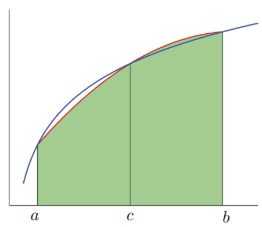
\includegraphics[width=0.5\textwidth]{images/simpson.png}
    \caption{Regla de Simpson}
    \label{fig:myplot18}
\end{figure}

\end{document}